% \section{Tujuan}
\section{Goals}
\begin{itemize}[label=$\bullet$, itemsep=-1pt, leftmargin=*]   
    % \item Mahasiswa mengerti tentang konsep pointer pada bahasa pemrograman C.
    \item Students are able to understand the concept of pointers in C.
    % \item Mahasiswa mengerti cara membuat dan memanggil struct pada bahasa pemrograman C.
    \item Students are able to create and call a struct in C.
    % \item Mahasiswa mengerti tentang algoritma sorting pada bahasa pemrograman C.
    \item Students are able to understand about sorting algorithm in C.
    % \item Mahasiswa mengerti tentang algoritma searching pada bahasa pemrograman C.
    \item Students are able to understand about searching algorithm in C.
    % \item Mahasiswa mampu mengaplikasikan konsep algoritma searching dan sorting pada bahasa pemrograman C.
    \item Students are able to apply the conceptof searching and sorting algorithm in C.
\end{itemize}

% \section{Pointer}
\section{Pointers}
% \subsection{Alamat Memori}
\subsection{Memory Address}
% Setiap variabel, fungsi, struct, ataupun objek lain yang dibuat dalam program mempunyai lokasi masing-masing pada memori. 
% Alokasi setiap variabel disimpan dalam alamat memori tertentu.
Every variables, functions, structs, or any object in a program have their own memory allocation. 
Said Allocations are saved in certain memory addresses

% Jika  terdapat variabel \verb|var| di program Anda, \verb|&var| akan memberi alamatnya di memori.
If there are any variable \verb|var| in your program, \verb|&var| will return its address in memory
\begin{lstlisting}[language=c]
    int var = 5;
    printf("%d\n", var);
    printf("%p\n", &var);
\end{lstlisting}
\begin{center}
	% \colorbox{pink}{\parbox{0.8\linewidth}{\textbf{Catatan:} Output bisa berbeda-beda di tiap eksekusi.}}
    \colorbox{pink}{\parbox{0.8\linewidth}{\textbf{Catatan:} Output may differ in each execution.}}
\end{center}

% \subsection{Pengenalan Pointer}
\subsection{Introduction to Pinters}

% Pointer(variabel penunjuk) adalah variabel khusus yang digunakan untuk menyimpan alamat, bukan nilai.
Pointers is a special variable that serves to save addresses, not value.

% Deklarasi variabel pointer menggunakan operator \verb|*| di antara tipe data dan nama variabelnya.
To declare a pointer variable, use \verb|*| operator between the data type and it's variable name.
\begin{lstlisting}[language=c]
	#include <stdio.h>
int main()
{
	int* p; // atau
    int * p2;
	return 0;
}
\end{lstlisting}


% \subsection{Cara Kerja Pointer}
\subsection{How Pointers Work}
% Berikut adalah cara kerja dari pointer.
The following is to show how pointers work.
% \begin{lstlisting}[language=c, caption={Contoh Program Pointer}]
\begin{lstlisting}[language=c, caption={Program Example}]
    #include <stdio.h>
    int main()
    {
       int* pc, c;
       
       c = 22;
       printf("Address of c: %p\n", &c);
       printf("Value of c: %d\n\n", c);  // 22
       
       pc = &c;
       printf("Address of pointer pc: %p\n", pc);
       printf("Content of pointer pc: %d\n\n", *pc); // 22
       
       c = 11;
       printf("Address of pointer pc: %p\n", pc);
       printf("Content of pointer pc: %d\n\n", *pc); // 11
       
       *pc = 2;
       printf("Address of c: %p\n", &c);
       printf("Value of c: %d\n\n", c); // 2
       return 0;
    }
\end{lstlisting}

Explanation:\\
\begin{enumerate}
    \item \verb|int* pc, c;|
    \begin{figure}[H]
        \centering
        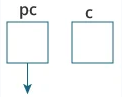
\includegraphics[width=0.2\linewidth]{../P4/img/screenshot001.png}
        \caption{}
        \label{fig:satu}
    \end{figure}
    \item \verb|c = 22;|
    \begin{figure}[H]
        \centering
        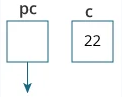
\includegraphics[width=0.2\linewidth]{../P4/img/screenshot002.png}
        \caption{}
        \label{fig:dua}
    \end{figure}
    \item \verb|pc = &c;|
    \begin{figure}[H]
        \centering
        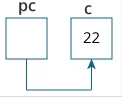
\includegraphics[width=0.2\linewidth]{../P4/img/screenshot003.png}
        \caption{}
        \label{fig:tiga}
    \end{figure}
    \item \verb|c = 11;|
    \begin{figure}[H]
        \centering
        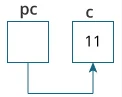
\includegraphics[width=0.2\linewidth]{../P4/img/screenshot004.png}
        \caption{}
        \label{fig:empat}
    \end{figure}
    \item \verb|*pc = 2;|
    \begin{figure}[H]
        \centering
        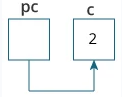
\includegraphics[width=0.2\linewidth]{../P4/img/screenshot005.png}
        \caption{}
        \label{fig:lima}
    \end{figure}
\end{enumerate}

\subsection{Double Pointer}
% Variabel pointer juga dapat menunjuk variabel pointer lainnya. 
% Hal ini disebut dengan double pointer (pointer to pointer). 
% Untuk mendeklarasikan variabel double pointer, digunakan dua simbol *. 
% Kegunaan paling umum dari variabel double pointer adalah untuk membuat array dua dimensi secara dinamis.
A pointer could also point to another pointer variable. This is called a double pointer (pointer to pointer).
To declare a double pointer, we use two \verb|*| operator between the data type and its variable name. 
The general usage of this double pointer variable is ti create a two dimensional array dinamically.
\begin{lstlisting}[language=c]
    int **dbPtr;
\end{lstlisting}
Variabel dbPtr di atas menyimpan alamat memori dari variabel pointer lainnya. \\
Berikut contohnya

The variable dbPtr above contains a memory address of another pointer variable.\\
Take a look at the example below.
% \begin{lstlisting}[language=c,  caption={Contoh Double Pointer}]
\begin{lstlisting}[language=c,  caption={Double Pointer Example}]
#include <stdio.h>

int main(void)
{
    int var = 23;
    int *ptr = &var;
    int **dbPtr = &ptr;

    printf("%d\n", **dbPtr);
        
    return 0;
}
\end{lstlisting}

% \subsection{Tugas Pendahuluan}
\subsection{Pre-lab Assignment}
\begin{enumerate}
%    \item Bagaimana cara mendeklarasikan pointer ke array multidimensi?
   \item Explain how to declare a pointer to a multidimensional array?
%    \item Buatlah program dalam bahasa C atau C++ yang mengimplementasikan 
%    fungsi void printMatrix(int **matrix, int rows, int cols) untuk mencetak matriks 2D menggunakan pointer ke pointer. 
%    Lalu, dalam fungsi main, buatlah matriks 2D dan panggil fungsi printMatrix untuk mencetak matriks tersebut.
   \item Create a program in C or C++ that implements void printMatrix(int **matrix, int rows, int cols) function
   to print out a 2D matrix using pointer to pointer. And then in the main function, create a 2D matrix and call the
   printMatrix function to print said matrix.
\end{enumerate}

\section{Struct}
% Dalam pemrograman C, struct (atau struktur) adalah kumpulan variabel (bisa dari tipe berbeda) di bawah satu nama. 
% Tidak seperti array yang hanya dapat menyimpan elemen dengan tipe data sama, 
% struct dapat mengelompokkan elemen dengan tipe data yang berbeda-beda.
In C, struct is a collection of variables (could be in various types) under one name. Unlike an array that could only
store elements with the same data type, struct is able to group elements with different data types.

% \subsection{Deklarasi Struct}
\subsection{Deklarasi Struct}
% Seperti variabel, struct harus dideklarasikan terlebih dahulu sebelum bisa digunakan. Pendeklarasian struct menggunakan sintaks 
% sebagai berikut.
Similar to variables, a struct must be declare first before use. Below is an example on how to declare a struct.

% \begin{lstlisting}[language=c]
% struct <nama_struct> {
%     <tipe_data_member> <nama_member>;
%     <tipe_data_member> <nama_member>;
%     <tipe_data_member> <nama_member>;
%     .
%     .
%     .
% };
% \end{lstlisting}
\begin{lstlisting}[language=c]
    struct <struct_name> {
        <member_dataType> <member_name>;
        <member_dataType> <member_name>;
        <member_dataType> <member_name>;
        .
        .
        .
    };
    \end{lstlisting}

Berikut adalah contoh deklarasi struct berdasarkan kasus Mahasiswa.
Below is a case example of struct declaration about students data.
% \begin{lstlisting}[language=c]
% struct Mahasiswa
% {
%     char *name;
%     char *address;
%     int age;
% };
% \end{lstlisting}
\begin{lstlisting}[language=c]
    struct Students
    {
        char *name;
        char *address;
        int age;
    };
    \end{lstlisting}
% \begin{center}
% 	\colorbox{pink}{\parbox{0.8\linewidth}{\textbf{Catatan:}  Menggunakan pointer * untuk data string}}
% \end{center}
\begin{center}
	\colorbox{pink}{\parbox{0.8\linewidth}{\textbf{Note:}  Use pointer * for string data type}}
\end{center}

% Setelah dideklarasikan, sebuah struct akan menjadi tipe data baru. 
% Maka dalam kasus ini, struct Mahasiswa di sini menjadi tipe data baru dengan member-member berupa \verb|nama|, 
% \verb|address|, dan \verb|age|. Untuk membuat variabel dengan tipe data struct, dilakukan dengan sintaks berikut.
After declaration, a struct will be its own data type. In this case, \textbf{Students} data type will be its own new data type
with members such as \verb|name|, \verb|address|, dan \verb|age|. Take a look at an example below to declare a variable
with the struct data type.

% \begin{lstlisting}[language=c]
%     struct <nama_struct> <nama_variabel>;
% \end{lstlisting}
\begin{lstlisting}[language=c]
    struct <struct_name> <variable_name>;
\end{lstlisting}

Example:
% \begin{lstlisting}[language=c]
%     struct Mahasiswa mhs1;
%     struct Mahasiswa mhs2;
% \end{lstlisting}
\begin{lstlisting}[language=c]
    struct Students mhs1;
    struct Students mhs2;
\end{lstlisting}
Contoh di atas menunjukkan terdapat dua variabel \verb|mhs1| dan \verb|mhs2 |bertipe struct \verb|Mahasiswa|.
The example above shows that there are two variables \verb|mhs1| and \verb|mhs2 with \verb|Mahasiswa| struct data type.

% \subsection{Akses Member Struct}
\subsection{Struct Member Access}
Bagaimana cara untuk mengakses member dari variabel struct yang telah dibuat? \\
Untuk mengakses member-member dari struct, digunakan operator dot (.) setelah nama variabelnya.
How do you access members from a struct variable? \\
To access members from a struct, we use a dot (.) operator after its variable name.

% \begin{lstlisting}[language=c]
%     <nama_variabel>.<member_struct>
% \end{lstlisting}
\begin{lstlisting}[language=c]
    <variable_name>.<member_name>
\end{lstlisting}

Example:
\begin{lstlisting}[language=c]
    mhs1.age = 20;
    mhs1.nama = iqbal;
    
    mhs2.nama = fatur;
    mhs2.age = 21;
\end{lstlisting}

\subsection{Pre-lab Assignment}
\begin{enumerate}
    % \item Buatlah sebuah struct yang merepresentasikan informasi tentang seorang mahasiswa, yang memiliki nama, nim, dan nilai IPK. 
    % Kemudian, buatlah program untuk menginput data mahasiswa, menampilkan data mahasiswa, dan menghitung rata-rata IPK dari 
    % sejumlah mahasiswa.
    \item Create a struct that represent informations about a students, the informations their name, student ID, and GPA.
    And then, create a program in insert student informations, display them, and calculate the average GPAs of a
    certain number of students
    \item Anda diberikan struct yang merepresentasikan titik dalam sistem koordinat dua dimensi (x, y). 
    Buatlah sebuah program C untuk menghitung jarak antara dua titik yang diinputkan oleh pengguna menggunakan rumus jarak Euclidean.
    \item Create a struct that represents coordinate points in a two dimensional plane (x,y). And then create a C program to calculate
    the distance between two points that a user inputs with a Euclidean formula. 
\end{enumerate}

% \section{Algoritma Sorting}
\section{Sorting algorithm}
% Sorting merupakan suatu proses penyortiran atau pengurutan sebuah data.\\
% Terdapat 2 macam pengurutan data pada sorting yaitu :
Sorting is a process of arranging or organizing data.\\
There are two types of data sorting, namely :
% \begin{enumerate}
%     \item Berdasarkan ascending (kecil ke besar).
%     \item Berdasarkan Descending (besar ke kecil).
% \end{enumerate}
\begin{enumerate}
    \item Ascending (small to large).
    \item Descending (large to small).
\end{enumerate}

\subsection{Bubble Sort}
% Bubble sort merupakan algoritma pengurutan yang membandingkan dua data yang berdekatan dan menukarnya sampai tidak dalam urutan 
% yang diinginkan. Bubble sort menggunakan teknik iterasi. Iterasi merupakan proses melakukan perulangan sebanyak data yang diketahui.
% Intinya pada iterasi melakukan perbandingan antara dua data.
Bubble sort is a sorting algorithm that compares two adjacent data points and swaps them until they are in the desired order. 
Bubble sort utilizes iteration method. iteration is a process of repeating a loop as many times as there is known data. 
Essentially, during each iteration, a comparison is made between two data points.

\begin{figure}[H]
    \centering
    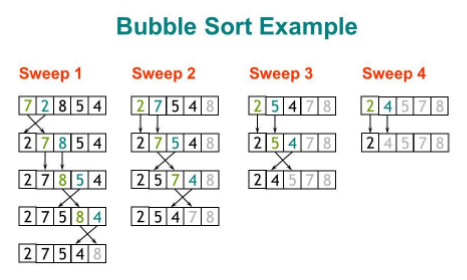
\includegraphics[width=0.7\linewidth]{../P4/img/screenshot006.png}
    \caption{}
    \label{fig:enam}
\end{figure}
% \begin{lstlisting}[language=c,caption=Implementasi Bubble Sort]
\begin{lstlisting}[language=c,caption=Bubble Sort Implementation]
void swap ( int * xp , int * yp ) {
   int temp = *xp;
   *xp = *yp;
   *yp = temp;
}

void bubbleSort(int arr[], int n) {
   int i, j, swapped;        // optimized with bool `swapped`:
   for (i = 0; i < n-1; i++) {
      swapped = 0;
      for (j = 0; j < n-i-1; j++) {
         if (arr[j] > arr[j+1]) {
            swap(&arr[j], &arr[j+1]);
            swapped = 1;
         }
      }
      if (swapped == 0)
         break;
   }
}
\end{lstlisting}

\subsection{Insertion Sort}
% Insertion sort merupakan teknik sorting dengan cara menyisipkan atau memasukan setiap elemen secara berulang berulang.
% Konsep insertion sort bisa diibaratkan sebuah kartu.
Insertion sort is a sorting technique that involves repeatedly inserting or placing each element. Imagine reshuffling a 
deck of cards to organize it.
\begin{figure}[H]
    \centering
    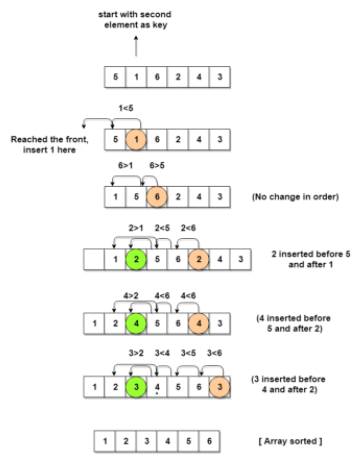
\includegraphics[width=0.5\linewidth]{../P4/img/screenshot007.png}
    \caption{}
    \label{fig:tujuh}
\end{figure}
% \begin{lstlisting}[language=c,caption=Implementasi Insertion Sort],
\begin{lstlisting}[language=c,caption=Insertion Sort Implementation], 
void insertionSort(int arr[]. int n) {
   int i, key, j;
   for (i = 1; i < n; i++) {
      key = arr[i];
      j = i-1;
    
      while (j >= 0 && arr[j] > key) {
         arr[j+1] = arr[j];
         j = j-1;
      }
      arr[j+1] = key;
   }
}
\end{lstlisting}

\begin{center}
	% \colorbox{pink}{\parbox{0.8\linewidth}{\textbf{Catatan:} Terdapat berbagai algoritma sorting lain. Pelajari secara mandiri}}
    \colorbox{pink}{\parbox{0.8\linewidth}{\textbf{Note:} There are other sorting algorithms. Look it up individually}}
\end{center}

% \subsection{Tugas Pendahuluan}
\subsection{Pre-lab Assignment}
\begin{enumerate}
    % \item Urutkan array berikut menggunakan algoritma Bubble Sort:

    % Array: [5, 2, 9, 1, 5, 6]
    \item Sort the following array using Bubble Sort:

    Array: [5, 2, 9, 1, 5, 6]
    \item Hitung kompleksitas waktu (Big O) dari algoritma Insertion Sort saat mengurutkan sebuah array dengan panjang n, 
    dan jelaskan bagaimana kompleksitas ini dihitung.
    \item Calculate the time complexity (Big O) of the Insertion Sort algorithm when soring an array of length n, and 
    explain how this complexity is calculated
\end{enumerate}

% \section{Algoritma Searching}
\section{Searching Algorithm}
% Searching merupakan proses pencarian sebuah data yang diinginkan.
Searching is a process of looking the desired data.

\subsection{Linear Search}
Linear Search bekerja dengan melakukan pengecekan kepada semua elemen yang ada.\\
Secara garis besar, cara kerja Linear Search adalah:

Linear Search works by checking all of the existing elements.\\
Essentially, the working principle of Linear Search is:

% \begin{enumerate}
%     \item Memeriksa item satu per satu.
%     \item Apabila ditemukan, maka “ketemu”.
%     \item Jika sampai akhir belum ditemukan, maka item yang dicari tidak ada.
% \end{enumerate}
\begin{enumerate}
    \item Checking items one by one.
    \item When it is found, the program will execute any statements that needs a condition of an item to be found.
    \item If the algorithm had checked every single data, then the desired item does not exist.
\end{enumerate}

% \begin{lstlisting}[language=c,caption=Implementasi Linear Search], 
\begin{lstlisting}[language=c,caption=Linear Search Implementation], 
int linearSearch(int arr[], int n, int item) {
    int i;
    for(i = 0; i < n; ++i) {
        if(item == arr[i])
          return 1;
    }
    return -1;
}
\end{lstlisting}   

\subsection{Binary Search}
% Binary Search adalah teknik pencarian di mana untuk setiap iterasinya kita membagi space pencarian menjadi hanya setengah 
% dari space pencarian awal hingga kita menemukan yang kita cari.
Binary Search is a searching technique where in each iteration we separate the searching space to half the initial searching space
until we find the desired item.

% \begin{lstlisting}[language=c,caption=Implementasi Binary Search],
\begin{lstlisting}[language=c,caption=Binary Search Implementation],   
bool f(int k, int a, int b, int n) {
   return ((k/a) * (b/a) >= n);
}

int binser(int a, int b, int n) {
   int l = 1;
   int r = 100000;
   while (r - l > 1) {
      int mid = (l + r) >> 1;
      bool can = f(mid);
      if(can)
         r = mid;
      else
         l = mid + 1;
   }
   if (can(l))
      return l;
   else
      return r;
}
\end{lstlisting}

\begin{center}
	% \colorbox{pink}{\parbox{0.8\linewidth}{\textbf{Catatan:} Terdapat berbagai algoritma searching lain. Pelajari secara mandiri}}
    \colorbox{pink}{\parbox{0.8\linewidth}{\textbf{Note:} There are other sorting algorithms. Look it up individually}}
\end{center}

% \subsection{Tugas Pendahuluan}
\subsection{Pre-lab Assignment}
\begin{enumerate}
    % \item Anda memiliki daftar nama berikut: ["Alice", "Bob", "Charlie", "David", "Eve", "Frank"]. 
    % Gunakan algoritma binary search untuk mencari apakah nama "Eve" ada dalam daftar ini. 
    % Jika ya, berapa langkah yang dibutuhkan?
    \item Given the following list of names: ["Alice", "Bob", "Charlie", "David", "Eve", "Frank"].
    Use the Binary Search algorithm to look for the name "Eve" in this list. If found, how many steps are required?
    % \item Jelaskan perbedaan antara pencarian linear (sequential search) dan pencarian biner (binary search).
    %  Kapan Anda akan memilih salah satu metode ini daripada yang lain?
    \item Explain the difference between Linear Search (Sequential Search) and Binary Search.
    in what scenario that you choose one method over the other?
\end{enumerate}
